Link to repo: \url{https://github.com/SkoogJacob/RedditDB}

See the following page for test results.
I used three different tests to load the data.
All tests were run in Java using a JDBC driver.
Loading of the unconstrained tables was done using multithreading, with each thread handling batches of 2000 records.

Loading the constrained tables was done on a single thread in batches of 15000 entries.

The test staging entries first to the unconstrained tables works just like the first test.
The only difference is that once the unconstrained tables are loaded it queries the SQL database to load all entries over to the constrained tables, trusting the SQL database to handle batching and multithreading.

The first tests, labelled "unconstrained" inserted the data into a table without any constraints.
This was the fastest to run, taking about 1.5 seconds on average to add all the entries.
This design does have the drawback of having an immense amount of duplicate records in the Redditor and Subreddit tables.

The second group of tests, labelled "constrained" was by far the slowest.
This is, in large part I believe, due to the code adding entries needing to check the database to avoid adding duplicate entries in the batches.
The execution speed would be even worse if the SQL server was run on a separate machine and all of these queries to avoid duplicates had to wait for network latency.
In addition, I was unable to use multithreading when adding entries to the heavily constrained table.

The last set of tests, labelled "test using staging to unconstrained tables" was much faster than the constrained tests, but it ends up with the same end results.
It does so by first adding all entries to the unconstrained tables as in the first round of tests.
It then queries SQL and asks it to add all distinct entries to the corresponding constrained table.

This test was run on the small file (90MB) which contains around 150--000 entries.

This last method will be the one I use to load in the actual database for the next part of the report.
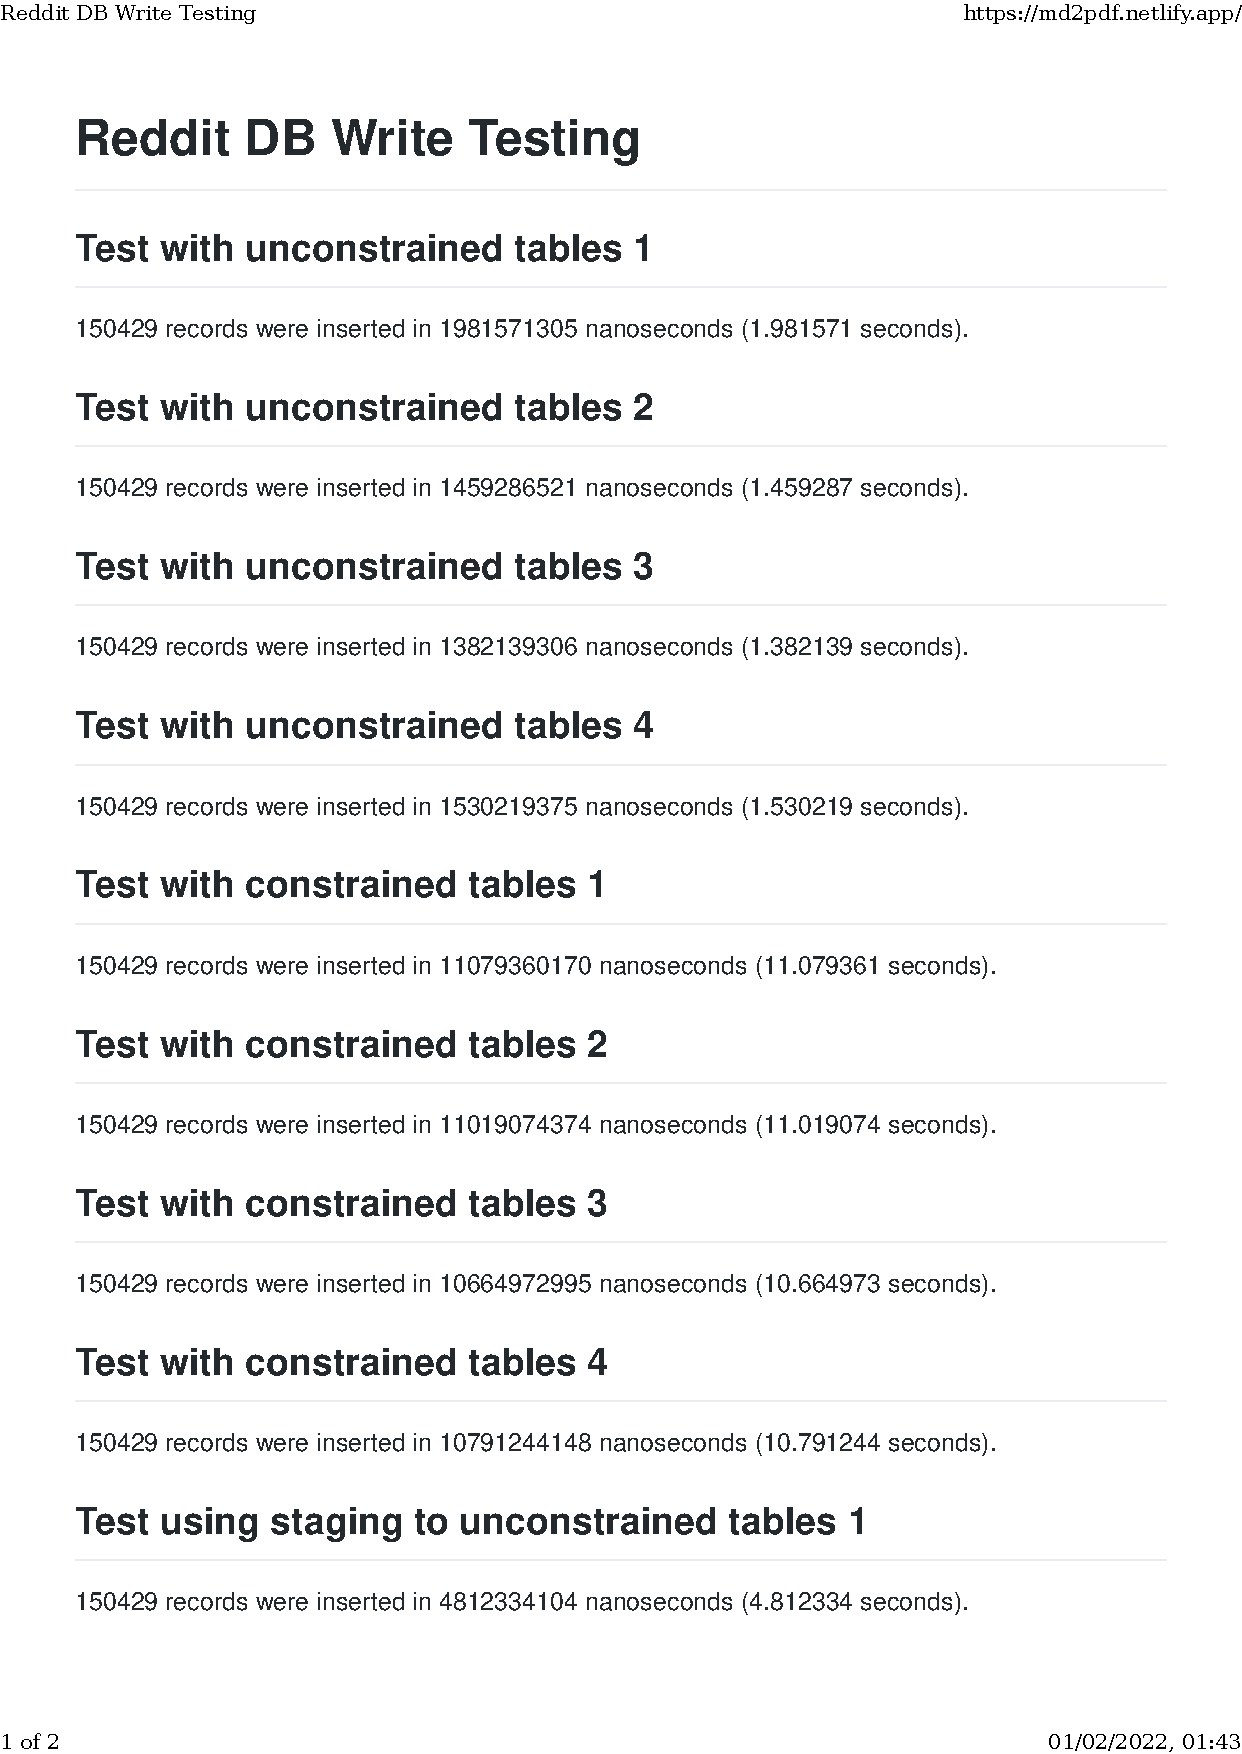
\includepdf[width=\textwidth, pages=-]{results.pdf}

After running this test I did some changes to the code and tried with adding most indexes and such after inserting the data into the table.
I did this because after inserting the entries from the 2012--12 file my database program was unable to drop the table if the indexes were still on it.
So I ended up modifying the loader code for the constrained table to insert with the bare minimum indexes active (only primary key and foreign keys).
I was also able to improve the code significantly and removed the need to query the database to avoid inserting duplicates into the redditor and
subreddits tables.
I was still unable to use multithreading, however, as it still led to conflicting locks (it added exactly 150--000 entries on the testing dataset, losing about 400 entries).

When trying to load the larger datasets I discovered that the code I used for staging was entirely broken for large datasets.
This is because the method I used required the entire source table being locked while it read from it.
But InnoDB has a default cap of around 6 million locked rows, so the 15GB dataset blew right past that.
To use the pre-staging test I would have to rewrite it to work in smaller batches.

The reason I will not implement this, though, is that after these improvements to loading the constrained table directly the staging table is no longer faster.
This is likely because the staging loader is simply doing more work than the constrained loader.
On the database side it is first doing the unconstrained loader and then the constrained loader afterwards, and the testing times are fairly consistent with this hypothesis.
Before the constrained loader had a huge inefficiency in that it was constantly querying the database to avoid inserting duplicates, so loading through a staging table ended up being faster just on virtue of not doing these redundant checks.
Now that that huge inefficiency is amended, there is no longer any advantage to using staging, at least not in the way that I implemented it.
Due to this I will simply abandon it and stick to my constrained loader.

I also significantly increased batch size for both the unconstrained and constrained loaders, as each comment having maximum body length was incredibly unlikely.
The batch sizes were increased to 6000 entries per batch for the unconstrained loader and 50--000 for the constrained loader.

The following two pages will have the results from loading the smaller test set as well as loading the large 2012--12 file.

\subsection{Conclusions}\label{subsec:loading_conclusions}

So, in total, adding the data first and then adding in the constraints afterwards seemed to offer the best performance when performing a large sequence of
operations.
This is because when the database has all the data loaded already, it can organize its work of indexing the data effectively.
When the indexes are already in place it is constantly re-ordering the table to abide by the index rules, and this constant reordering is quite expensive.

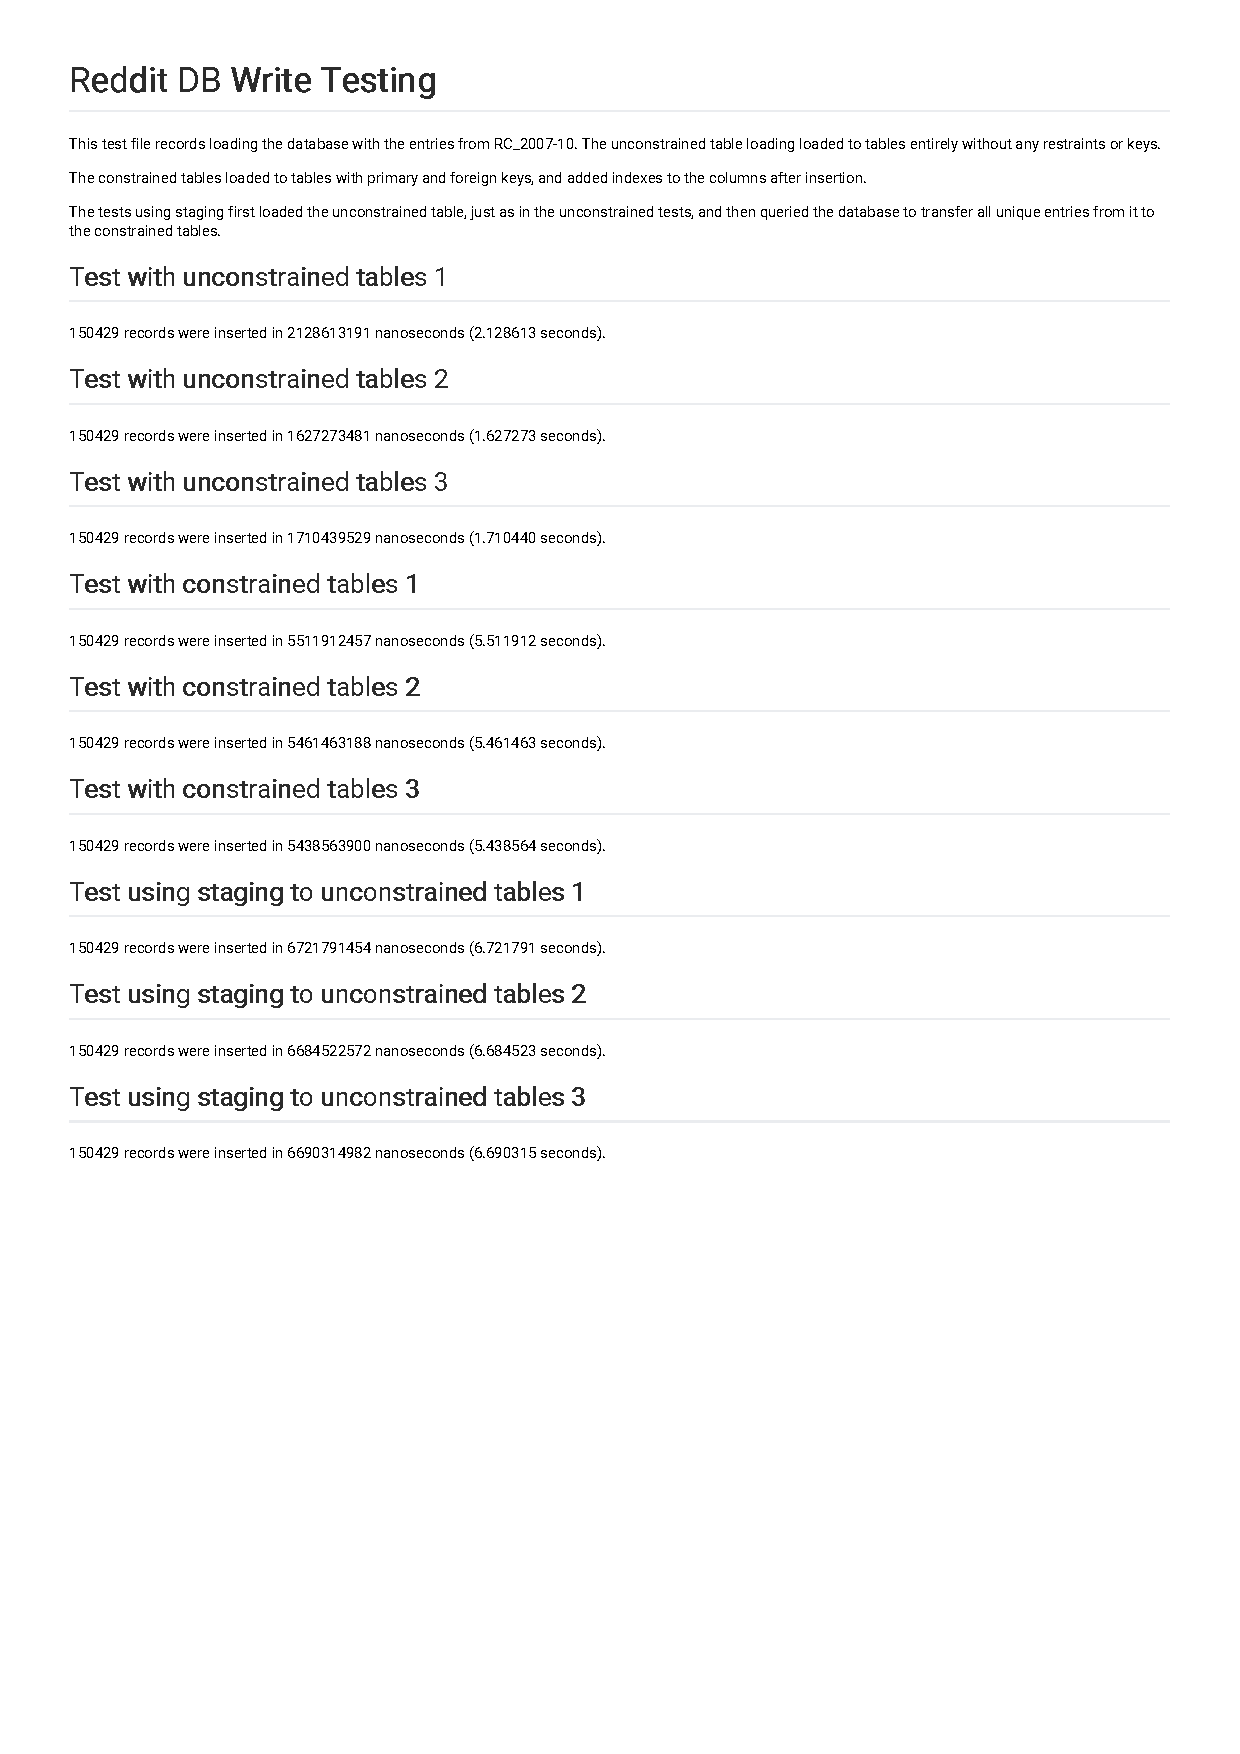
\includepdf[width=\textwidth, pages=-]{report_improved.pdf}
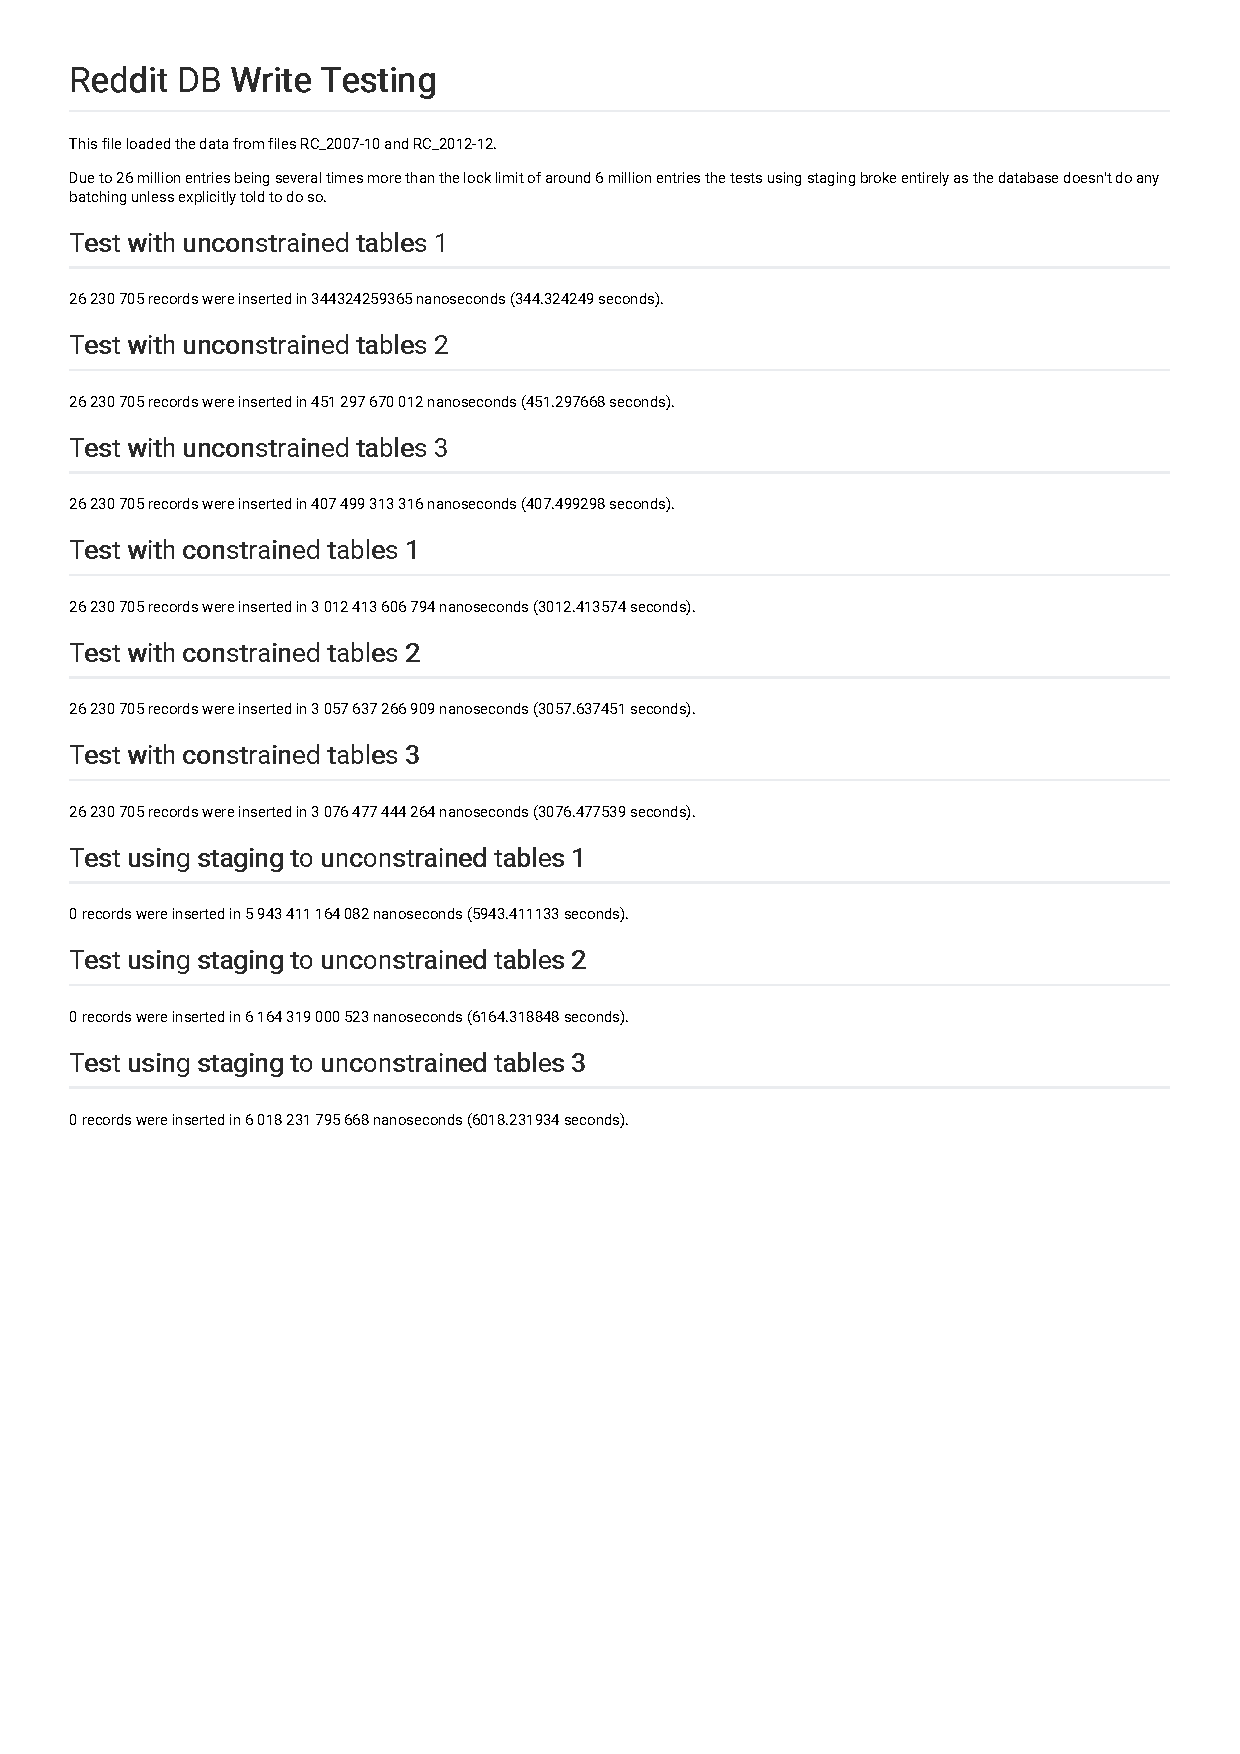
\includepdf[width=\textwidth, pages=-]{report_improved_big_data.pdf}